\chapter{Evaluation}
\label{eval}

% With the prototype implementation, we conduct extensive evaluation including 
% system/network-wide benchmarks. 

\begin{table}[htb]%\scriptsize
	\begin{minipage}{.47\linewidth}
		\caption{Benchmark results for the transfer policy lookup (ns).}
		\label{tab:authorization}
		\begin{tabularx}{1\linewidth}{X|XX}
			\toprule
			\# of Policies & Cache Hit & Cache Miss \\
			\midrule
			100            & 307       & 236        \\
			\SI{1}{K}      & 405       & 264        \\
			\SI{10}{K}     & 423       & 293        \\
			\SI{100}{K}    & 497       & 375        \\
			\bottomrule
		\end{tabularx}
	\end{minipage}
	\begin{minipage}{.47\linewidth}
		\caption{Key derivation times for different network sizes (ns).}
		\label{tab:derivation}
		\begin{tabularx}{1\linewidth}{X|XX}
			\toprule
			\# of Branches & 1st-level Key & 2nd-level Key \\
			\midrule
			% 10		& 189 	& 122 \\	% 841-530-189=122
			100            & 199           & 116           \\	% 845-530-199=116
			\SI{1}{K}      & 211           & 136           \\	% 877-530-211=136
			\SI{10}{K}     & 238           & 201           \\	% 969-530-238=201
			\SI{100}{K}    & 427           & 154           \\	% 1111-530-427=154
			\bottomrule
		\end{tabularx}
	\end{minipage}\vspace{2em}
	\begin{minipage}{.47\linewidth}
		\caption{Processing times for the encryption/decryption for different packet sizes (ns).}
		\label{tab:authentication}
		\begin{tabularx}{1\linewidth}{X|XX}
			\toprule
			Packet Size (byte) & Encryption & Decryption \\
			\midrule
			100                & 856        & 659        \\
			500                & 1082       & 747        \\
			1000               & 1338       & 850        \\
			1500               & 1557       & 950        \\
			\bottomrule
		\end{tabularx}
	\end{minipage}
\end{table}

\begin{figure}
	\begin{minipage}{.47\linewidth}
		\centering
		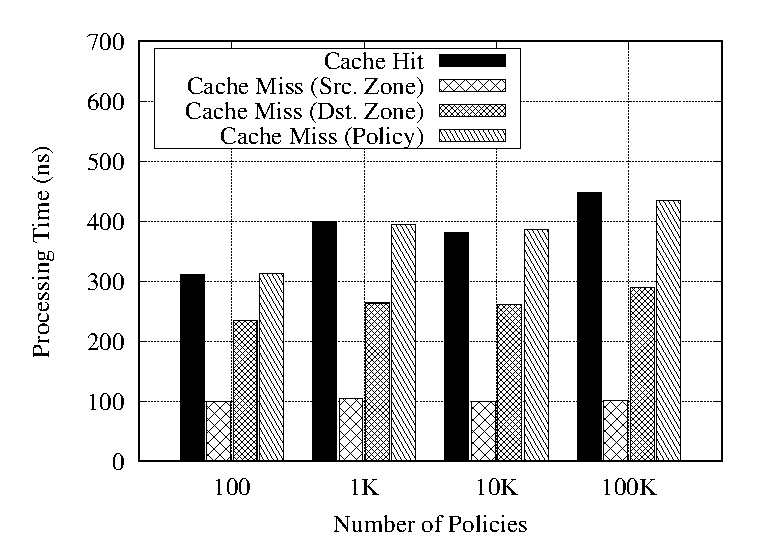
\includegraphics[width=\linewidth]{intra_domain.eps}
		\caption{Processing time for intra-domain zone transfer.}
		\label{fig:intra}
	\end{minipage}\hspace{1em}
	\begin{minipage}{.47\linewidth}
		\centering
		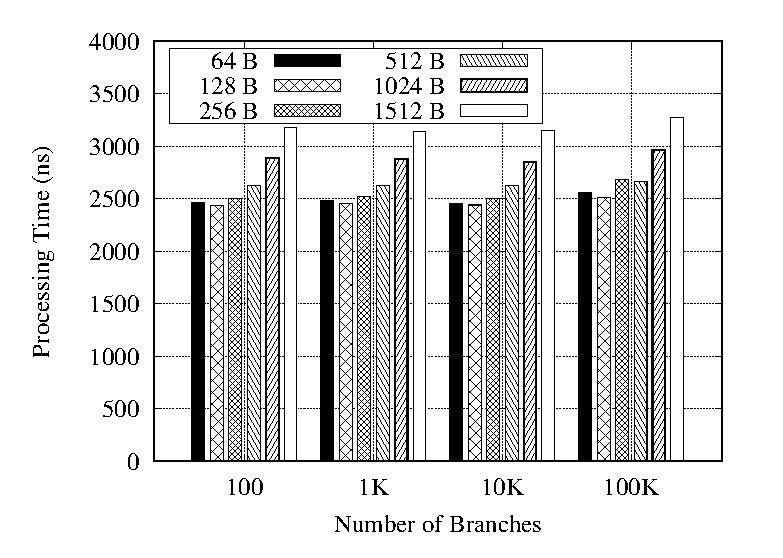
\includegraphics[width=\linewidth]{inter_sender.eps}
		\caption{Processing time on $TP_S$ for inter-domain zone transfer.}
		\label{fig:inter_sender}
	\end{minipage}\vspace{2em}
	\begin{minipage}{.47\linewidth}
		\centering
		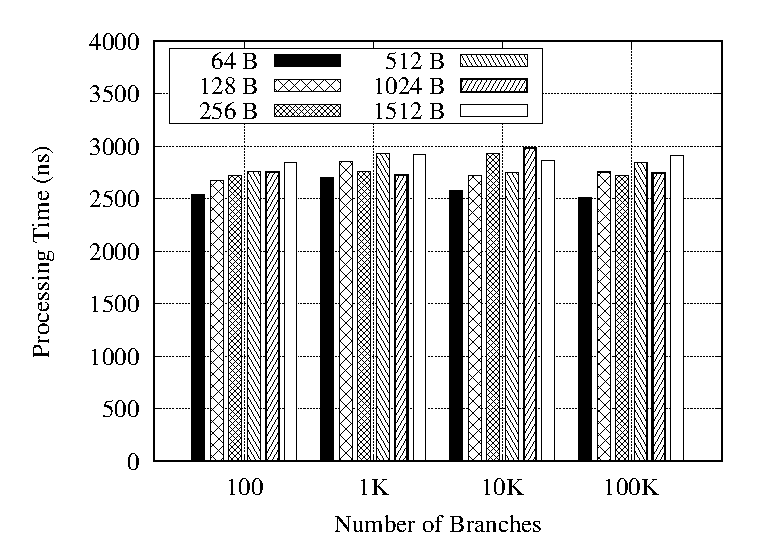
\includegraphics[width=\linewidth]{inter_receiver.eps}
		\caption{Processing time on $TP_R$ for inter-domain zone transfer.}
		\label{fig:inter_receiver}
	\end{minipage}\hspace{1em}
	\begin{minipage}{.47\linewidth}
		\centering
		\includegraphics[width=\linewidth]{pps.eps}
		\caption{Forwarding performance of \tp for various size of packets.}
		\label{fig:forwarding}
	\end{minipage}\vspace{2em}
	\begin{minipage}{.47\linewidth}
		\centering
		\includegraphics[width=\linewidth]{cdf_goodput.eps}
		\caption{CDF of goodput for 1400-bytes of maximum segment size (MMS).}
		\label{fig:goodput}
	\end{minipage}\hspace{1em}
	\begin{minipage}{.47\linewidth}
		\centering
		\includegraphics[width=\linewidth]{cdf_throughput.eps}
		\caption{CDF of throughput including extra header fields.}
		\label{fig:throughput}
	\end{minipage}
\end{figure}

\section{System Benchmarks}
\label{sec:systembenchmark}

% \paragraph{Experimental Setup}
We first conduct microbenchmark tests to evaluate the performance of \tp including the key
derivation, packet authentication, and authorization. For scrutinize and reproducible evaluation,
we leverage the standard benchmark library \texttt{testing} officially supported by golang.
The benchmarks are conducted on commodity machines equipped with an Intel i7 \SI{2.9}{GHz}
CPU, \SI{16}{GB} memory, and a \SI{1}{GbE} NIC.

\paragraph{Authorization}
% The \tp's transfer module performs zone transfer authorization for every incoming packets.
From technical perspectives, the zone transfer authorization is a database lookup consisting
of three tree searches;
upon receiving the packet metadata from the core module, the transfer module first looks
up the corresponding zone identifiers for the source and destination addresses, and then
compares them to the zone transfer policies. The authorization performance is therefore
dependent on the lookup time for the policy database.

Table~\ref{tab:authorization} shows
the benchmark results of database lookups for different quantities of policies.
Note that each benchmark ran a couple million iterations and kept the mean value.
The authorization check takes approximately 300 to \SI{500}{ns} per packet, which is a
notable result considering: i) a single lookup consists of three tree searches, ii) the result
is from a high-level language implementation, and iii) the test set scales 1000 times.
As expected, a lookup failure is commonly 24 to 31~\% faster than a successful lookup.
This implies that abnormal packets with invalid zone transfer requests can be quickly
discarded.


\paragraph{Key Derivation}
% When a \tp handles an inter-domain zone transfer packet, the \tp need to derive a correct 
% key for the authentication. As we described in~\S\ref{ssec:keymanagement}, the key derivation
% comprise with two steps: fetch the first-level key from the cache, and dynamically derive the 
% second-level key from the first-level key. 
% To securely forward a zone transfer packet over the public Internet, a \tp first 
We investigate the key derivation performance. Recall that the key derivation proceeds
differently for sender and receiver. Since the receiver is capable of directly deriving the
second-level key from the local secret which is relatively faster than sender-side key
derivation, here we focus primarily on the sender-side key derivation which comprises two steps;
fetching the first-level key from the key table (Eq.~\ref{eq:1stkey}) and deriving the
second-level key from the first-level key (Eq.~\ref{eq:2ndkey}). From a scalability
perspective, we vary the number of branches (a \tp for each) by increasing the number of stored
first-level keys up to \SI{100}{K}. Table~\ref{tab:derivation} depicts the average results of
benchmark tests iterated over a million times each.
% \claude{what about receiver side key derivation?}

We observe that the lookup time for the first-level key is independent of the size of the key
table, taking between \SI{154}{ns} and \SI{161}{ns}. In addition, the size of the key table is
also irrelevant for the second-level key derivation
because second-level keys are directly derived from first-level keys.
The results indicate that the processing time for a key derivation is less than 1 $\mu$s
even in very large networks with \SI{100}{K} branch sites, which is negligible considering
network latency in today's Internet.
% ---$\Delta t = \delta t_{Init} + \delta t_{1} + \delta t_{2}$.


\paragraph{Authentication}
The additional processing time for packet encryption and decryption is shown in
Table~\ref{tab:authentication}. In summary, it requires approximately 1.5 to 2.5 $\mu$s to
authenticate various sizes of packets. We note that the processing overhead occurs for the majority
of tunneling technologies that provide confidentiality for data transmission. The processing
time can be minimized with implementations using the Data Plane Development Kit (DPDK)~\cite{dpdk} or by leveraging hardware dedicated to cryptographic operations.


% \begin{figure*}[!htb]
% 	\begin{minipage}{.32\linewidth}
% 		\centering
% 		\includegraphics[width=\linewidth]{figs/pps.eps}
% 		\caption{Forwarding performance of \tp for various size of packets.}
% 		\label{fig:forwarding}
% 	\end{minipage}\hspace*{1em}
% 	\begin{minipage}{.32\linewidth}
% 		\centering
% 		\includegraphics[width=\linewidth]{figs/cdf_goodput.eps}
% 		\caption{CDF of goodput for 1400-bytes of maximum segment size (MMS).}
% 		\label{fig:goodput}
% 	\end{minipage}\hspace*{1em}
% 	\begin{minipage}{.32\linewidth}
% 		\centering
% 		\includegraphics[width=\linewidth]{figs/cdf_throughput.eps}
% 		\caption{CDF of throughput including extra header fields.}
% 		\label{fig:throughput}
% 	\end{minipage}
% \end{figure*}

\section{Network Benchmarks}
\label{sec:networkbenchmark}

So far, we evaluated the performance of each instruction newly introduced. Since a different
set of instructions needs to be applied depending on the zone transfer usecase, it is also
important to investigate the overall network performance for handling different types of zone
transfer packets. We now benchmark the actual network performance for both intra-/inter-domain
zone transfer cases.

\paragraph{Latency Inflation}
Figure~\ref{fig:intra} illustrates the network benchmark results for the intra-domain zone
transfer where the source and destination zones are within the same local network, such that
the \tp only performs zone transfer authorization. Since no cryptographic operations are involved,
the additional latency is negligible (as a single legitimate zone transfer takes $\sim$
\SI{500}{ns}). There might be an authorization abort due to a lookup failure that could be
caused by the following three reasons: no source zone ID, destination zone ID, or
zone transfer policy. In our prototype, the lookups are performed sequentially and thus
there are different processing overheads (\SI{100}{ns} $\sim$ \SI{600}{ns}) depending on when a
lookup failure occurs. Nevertheless, in case there exists no valid zone-transfer policy, the
packet will be simply dropped and therefore no additional latency is caused.

For inter-domain zone transfer cases, we benchmark the overall network inflation during \tp
operations including packet parsing, key derivation, authorization, and authentication.
Figure~\ref{fig:inter_sender} and~\ref{fig:inter_receiver} depict the processing delay from
sender-side \tp and receiver-side \tp, respectively.
From the results, we make the following observations: first, the overall latency inflation that
\name introduces is insignificant ($\sim 3 \mu$s). Second, \name scales well with the size of the
network, i.e., the number of branches. We do not see any notable performance degradation
($\leq$ \SI{200}{ns}). Third, the size of a packet is the primary factor for the latency increment
as expected for all data-plane devices. The packet size has a small latency incremental factor of
1.28 (i.e, 2.4 $\mu$s to 3.8 $\mu$s). Lastly, we observe no significant bias in network
performance between sender-side and receiver-side \tps.


\paragraph{Forwarding Performance}
We further investigate the actual forwarding performance for various packet sizes (\SI{128}{B},
\SI{256}{B}, \SI{512}{B}, \SI{1024}{B}) including a representative mixture of Internet traffic
(iMIX)~\cite{rfc6985}; we select the minimum packet size of 128 bytes instead 64 bytes which is
commonly considered to be the smallest packet size, because \name's tunneling requires at least 116
bytes long frame, i.e., Outer L3 header (40 bytes), AT header
(36 bytes), and EIP (40 bytes). Figure~\ref{fig:forwarding} shows the results. The
baseline is the forwarding performance without \tp operations. The other bars represent the
forwarding performance for intra-domain zone transfer (with authorization only) and inter-domain
zone transfer (with authorization and authentication) respectively.

For 128-byte packets which demonstrates the highest packet rate, and thus requiring the most
extreme packet processing, the intra-domain zone transfer exhibits a throughput degradation
of only 11\%. It also achieves 97 $\sim$ 100 \% of throughput for other packet sizes. These
results are expected because the \tp performs only authorization for the intra-domain zone
transfer packets, which would increase a processing delay of $\leq$ 500 ns; considering that
a typical intra-domain packet transmission used to show a few milliseconds of latency, the
additional delay is negligible.

On the other hand, the inter-domain zone transfer degrades the throughput by 44\% for the
smallest packets. Although the degradation diminishes as the packet size increases, the
performance still degrades by 24\% for the iMIX traffic. To investigate the main degradation
factor, we compare the amount of transmitted data (goodput) and the total bits transmitted
including all the network headers (throughputs) as shown in Figure~\ref{fig:goodput} and
\ref{fig:throughput}. From the comparison, we observe the followings: i) the inter-domain
zone transfer achieves a similar throughput to the baseline if the extra headers are considered,
ii) the performance degradation is caused by not only the additional processing delay but also
transmission delay of the extra headers, and therefore iii) \name performs similar to the
today's tunneling applications while providing the security policy enforcement for network
zoning.



% \subsection{Overhead Measurements}
% \label{ssec:overhead}

% \paragraph{Bandwidth Overhead}

% \paragraph{Memory Overhead}

% \paragraph{Control-plan Overhead}

